\documentclass[acmtog]{acmart}
\usepackage{graphicx}
\usepackage{subfigure}
\usepackage{natbib}
\usepackage{listings}
\usepackage{bm}
\usepackage{amsmath}

\usepackage{listings}
\lstset{
    columns = fixed,
    basewidth = {0.5em},
    breaklines = true,
    backgroundcolor = \color{white},
    keywordstyle = \color[RGB]{40, 40, 255},
    numberstyle = \footnotesize\color{darkgray},
    commentstyle = \ttfamily\color{violet},
    basicstyle = \ttfamily,
    stringstyle = \ttfamily\color[RGB]{128, 0, 0},
    showstringspaces = false,
    language = {[11]C++},
    escapechar = \@
}
\lstnewenvironment{cpp}[1][]{\lstset{language = {[11]C++}, #1}}{}

\definecolor{blve}{rgb}{0.3372549 , 0.61176471, 0.83921569}
\definecolor{gr33n}{rgb}{0.29019608, 0.7372549, 0.64705882}
\makeatletter
\lst@InstallKeywords k{class}{classstyle}\slshape{classstyle}{}ld
\makeatother
\lstset{language=C++,
	basicstyle=\ttfamily,
	keywordstyle=\color{blve}\ttfamily,
	stringstyle=\color{red}\ttfamily,
	commentstyle=\color{magenta}\ttfamily,
	morecomment=[l][\color{magenta}]{\#},
	classstyle = \bfseries\color{gr33n}, 
	tabsize=2
}
\lstset{basicstyle=\ttfamily}

% Title portion
\title{Final Project:\\ {Massive rigid-body simulation}} 

\author{Group:\quad 27 \\ Member:\quad YE HENGWEI \quad SHAO KUIXIANG  }

% Document starts
\begin{document}
\maketitle
\Large
\vspace*{2 ex}
\begin{figure}[htb]
	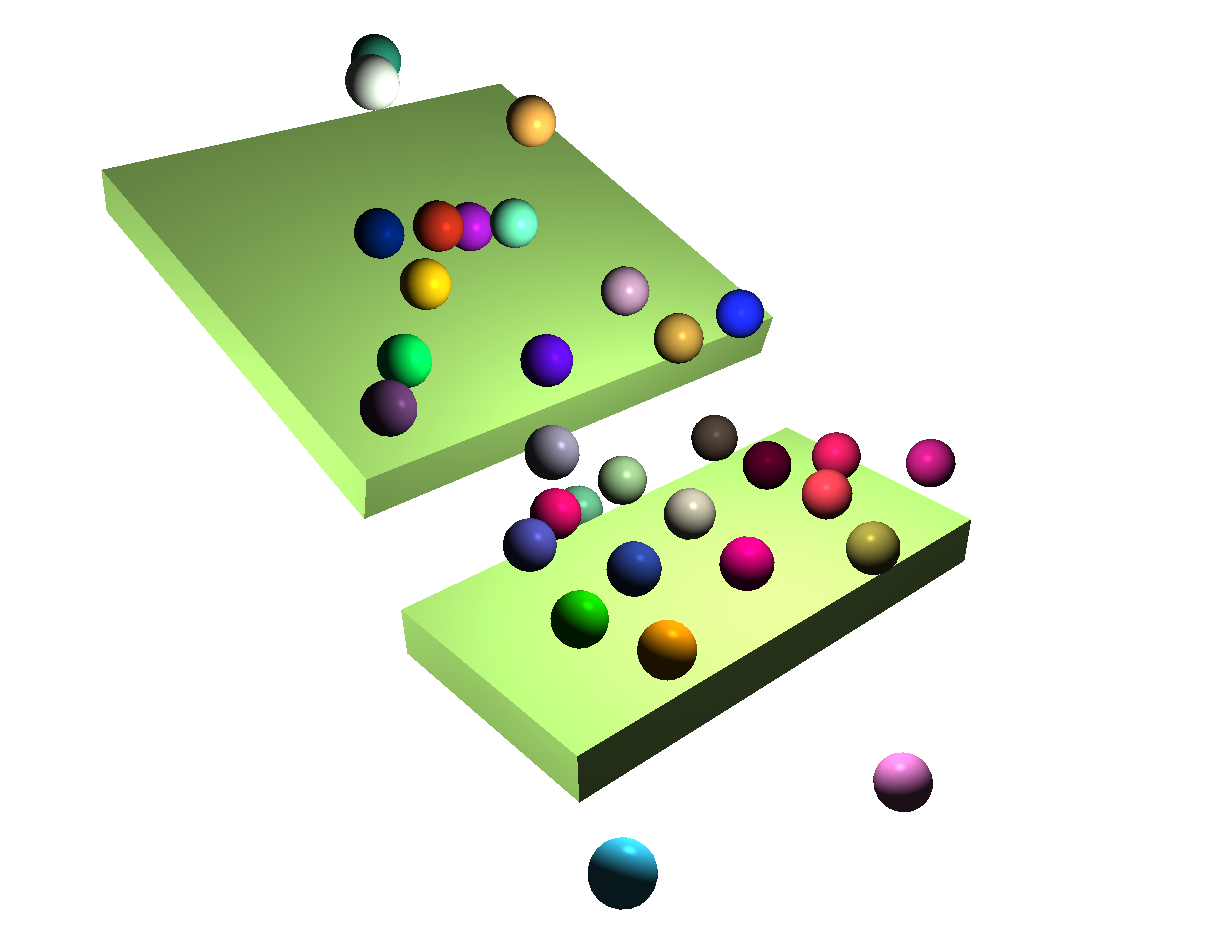
\includegraphics[width=\linewidth]{banner.png}
\end{figure}
\section{Introduction}
A Rigid Body is a concept in Kinematic and refers to an object which remains the same shape, size, and relative position of its internal points during motion and under force. In animation, rigid body give kinematic properties to objects, such as mass, drag and angular drag. Without rigid body, objects may penetrate each other withou colliding.\\
Our project aims to implement basic rigid body effects on objects and simulate the interaction of a masive number of rigid bodies within the physical world. The part of our implementation is mainly divided into three modules:
\begin{enumerate}
	\item Scene Initialization: A good scene can better reflect the interaction effect of rigid bodies, we mainly use opengl to render the entire scenes and generate our testing objects.
	\item Collision Detection: Whether there is contact between any two objects is a prerequisite for checking collision, we use AABB to preliminaries determine this between rigid bodies, and then further check the collision point.
	\item Collision Handling: After determining the collision, we use the impulse method to simulate and calculate the change of the rigid body's velocity and angular velocity, and then update the position and rotation of the object.
\end{enumerate}
\begin{figure}[htb]
	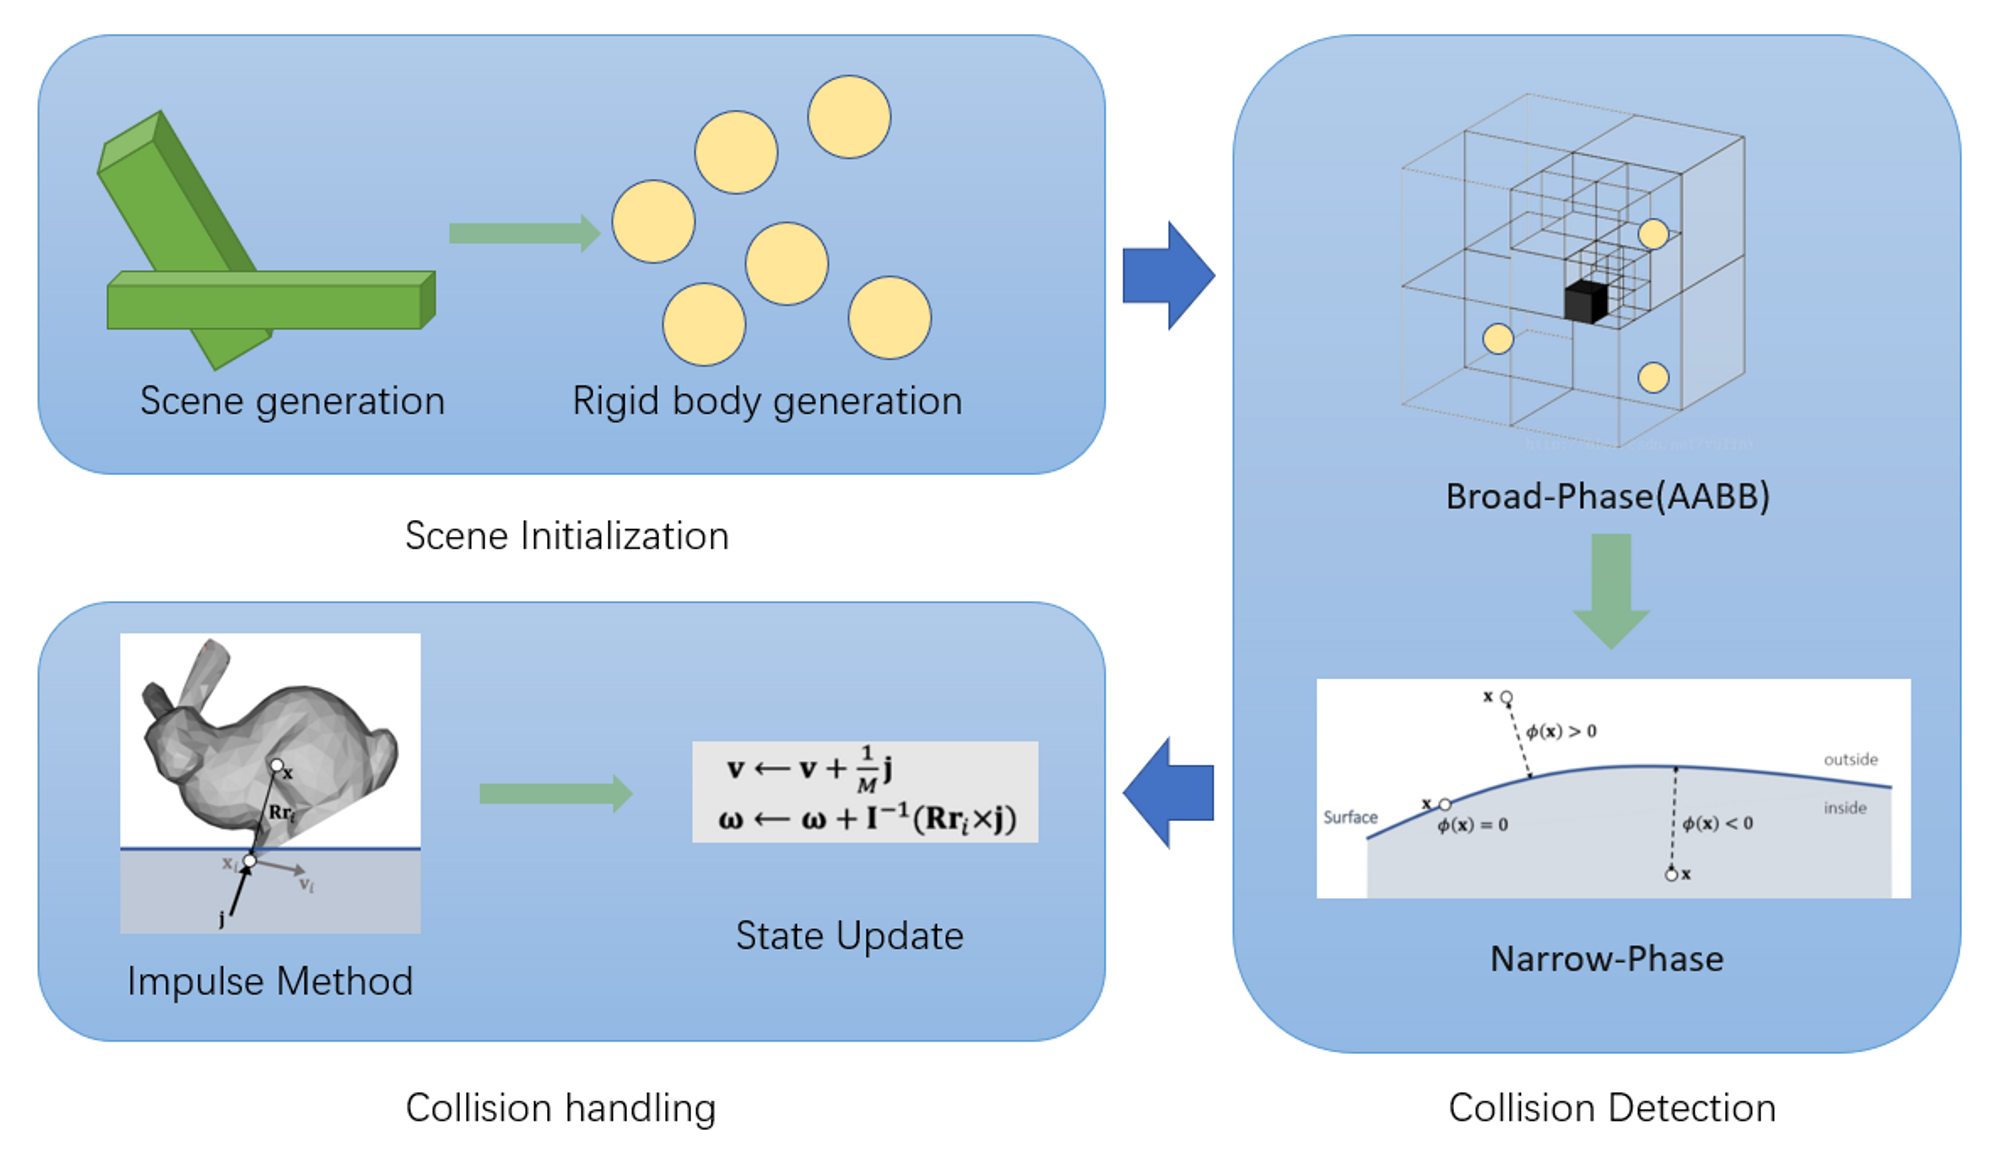
\includegraphics[width=\linewidth]{Introduction.png}
	\caption{Pipeline}
\end{figure}
\section{Scene Initialization}
\subsection{Scene Generation}
The objects we need include the wall class as a scene and the ball and bunny classes as movable rigid bodies.With the bunny class we have implemented the import of complex geometry.On this basis, we implement custom editing of the scene and the definition of the initial state of the object, so that we can generate any animation effect we want.
\subsection{Rigid body Generation}
A rigid body has four states: position $x$, rotation $q$, velocity $v$, and angular velocity $w$. Rigid body dynamics studies how to update these four states of a rigid body under the action of a force.
\begin{figure}[htb]
	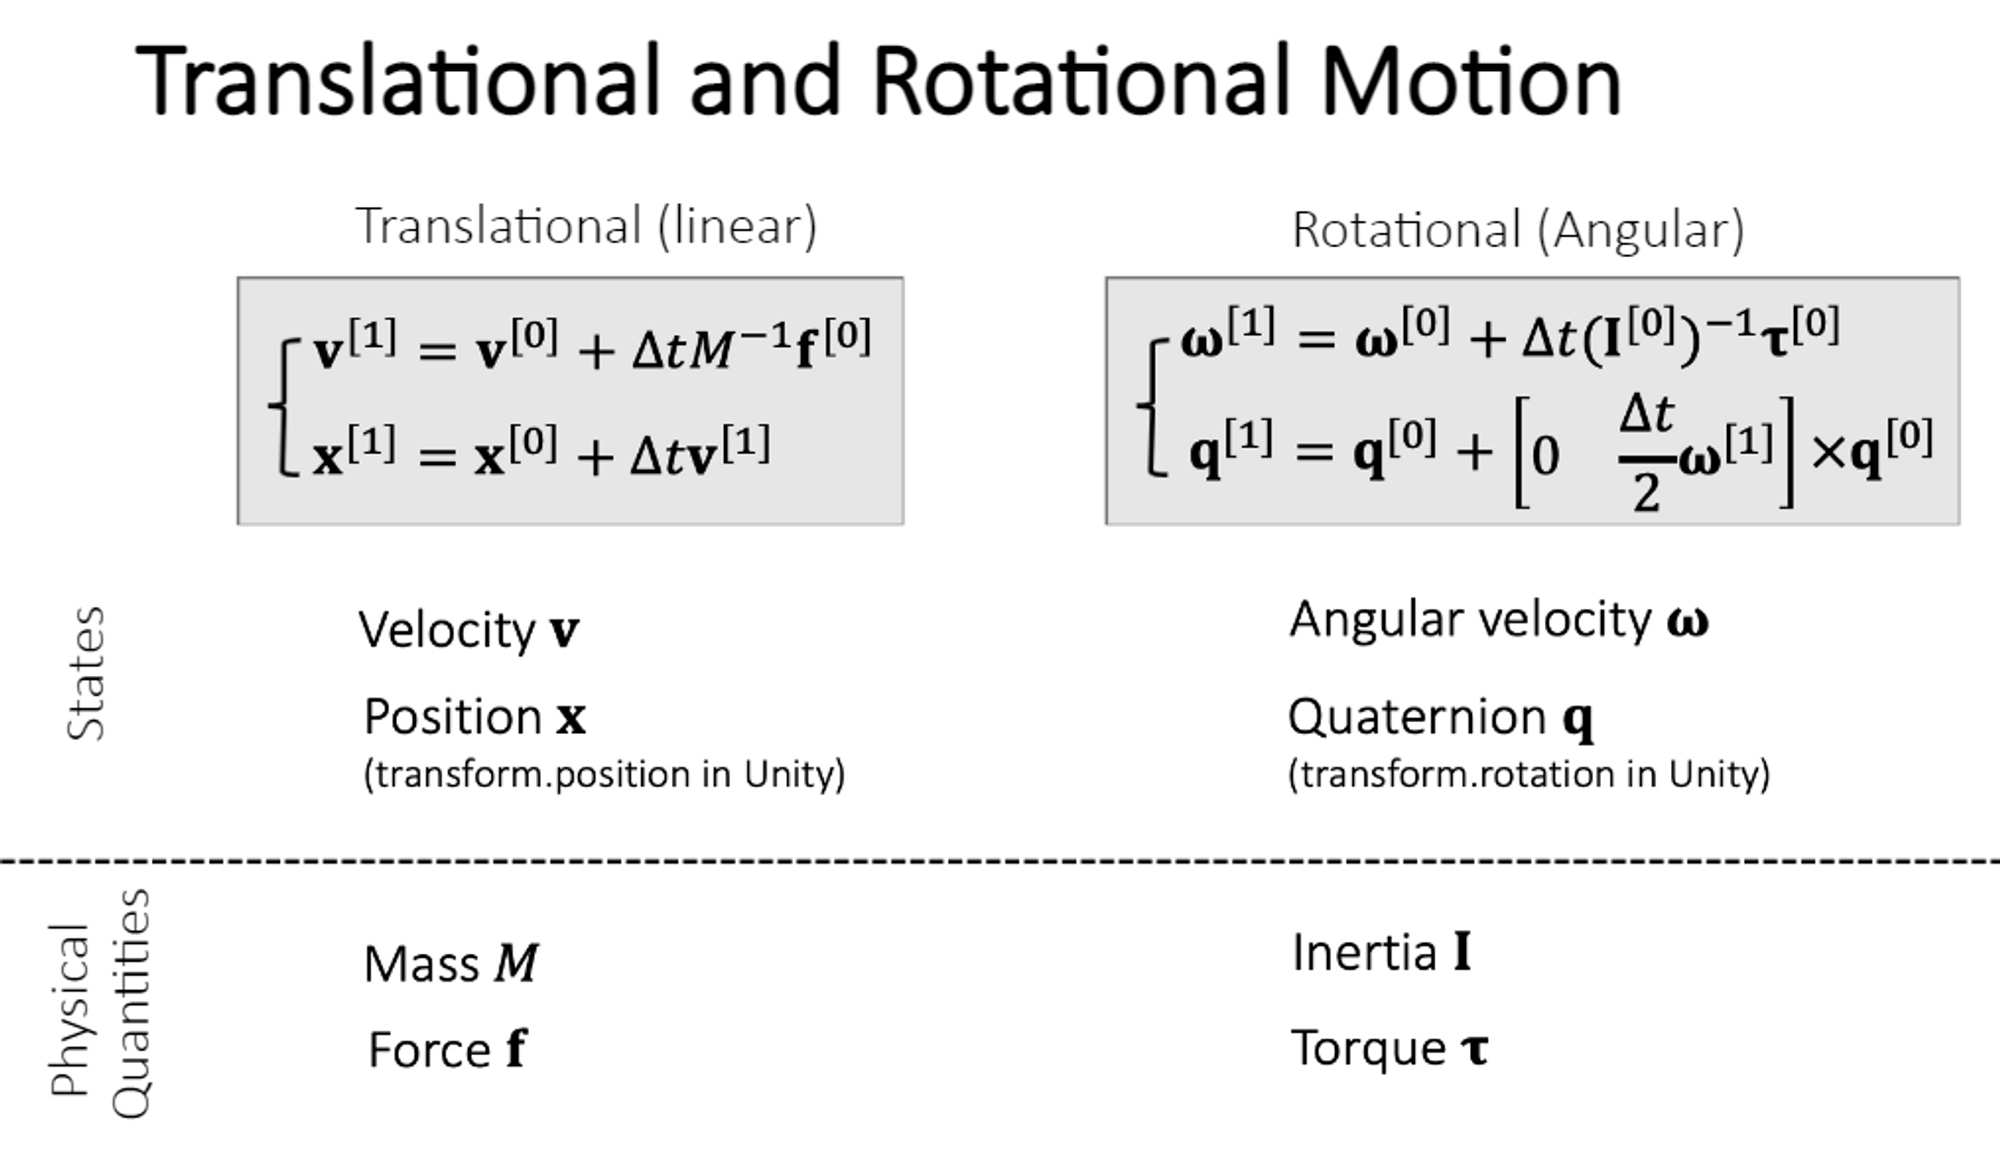
\includegraphics[width=\linewidth]{Rigid Body Dynamics.png}
	\caption{Rigid Body Dynamics}
\end{figure}
\subsubsection{Translation Dynamics}
The physical principle of translational dynamics, known as Newton's second law: $F=ma$, is that if we know the force and the mass of the object, we can directly calculate the acceleration, and then get the velocity and position.\\
But in programming practice, integrals can only be computed discretized. At each small time step, we consider the velocity to be constant.
\subsubsection{Rotation Dynamics}
The same as mass in linear dynamics, we need a variable that represents the tendency of the object to resist rotation, which is called intertia tensor and we need a 3x3 matrix to represent it.\\
Calculating intertia tensor requires viewing the object as a series of dots, when the object is static, $I_{ref}=\sum m_i(r_i^Tr_i1-r_ir_i^T)$, where $m_i$ is the dot's mass, $r_i$ is the vector from particle to this dot and $1$ is a 3x3 unit matrix.\\
When the object is rotated, the new intertia tensor is going to be $I=RI_{ref}R^T$.
\begin{cpp}
class Mesh{
	Vec3 v; // velocity
	Vec3 w; // angular velocity
	Mat3 I_ref; // intertia tensor
	float mass; // mass
}
\end{cpp}
\section{Collision Detection}
Imagine a scene with N objects. If we were to detect collisions between every two of these objects, the computational complexity would be $O(N^2)$, which is obviously not acceptable for a computer, so we need to do a preliminary screening before dealing with collisions between points. 
\subsection{Broad Phase(AABB)}
\begin{figure}[htb]
	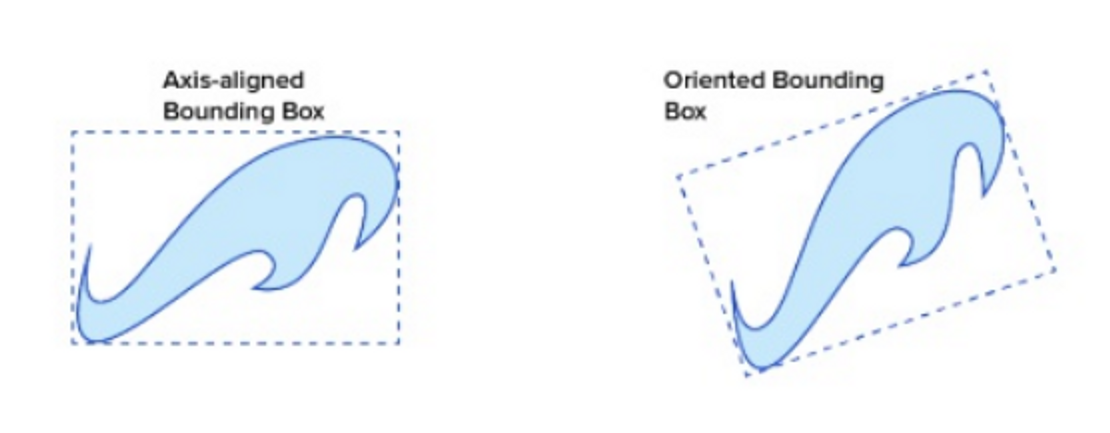
\includegraphics[width=\linewidth]{AABB.png}
	\caption{AABB}
\end{figure}
The basic idea we use is creating some bounding volumes(AABB) to represent the collision information of rigid bodies.
\begin{cpp}
struct AABB {
	Vec3 low_bnd;
	Vec3 upper_bnd;

	AABB() : low_bnd(0, 0, 0), upper_bnd(0, 0, 0) {};
	AABB(Vec3 center) {};

	Vec3 getCenter() {}
	bool intersect(struct AABB& aabb) {}
	bool containPoint(const Vec3& point) const{}
};
\end{cpp}
Represents the AABB information of a rigid body, which needs to save the maximum and minimum points. To determine whether two AABBs intersect, it is sufficient to determine whether both AABBs have overlapping parts in each axis. (The maximum number of balls simultaneously are compared below.)
\begin{table}[htb]
	\begin{tabular}{|c|c|c|c|l}
	\cline{1-4}
			 & Scene 1 & Scene 2 & Scene 3 &  \\ \cline{1-4}
	Base     & 25      & 26      & 26      &  \\ \cline{1-4}
	Distance & 100     & 130     & 115     &  \\ \cline{1-4}
	AABB     & 125     & 135     & 140     &  \\ \cline{1-4}
	\end{tabular}
	\caption{Maximum number of balls simultaneously}
\end{table}
\\\\\\\\\\Although the AABB intersection test is fast, we still can't test two objects against each other, so we need some spatial partitioning to reduce the number of intersection tests like BVH and BSP tress. However, due to limited time, we have not completed it yet.
\subsection{Narrow Phase(SDF)}
The signed distance function $\phi(x)$ is the shortest signed distance between a point and the target geometry, and it is very suitable for collision detection, indicating that the point is inside the geometry (collision), and the point is outside the geometry (no collision).
\begin{figure}[htb]
	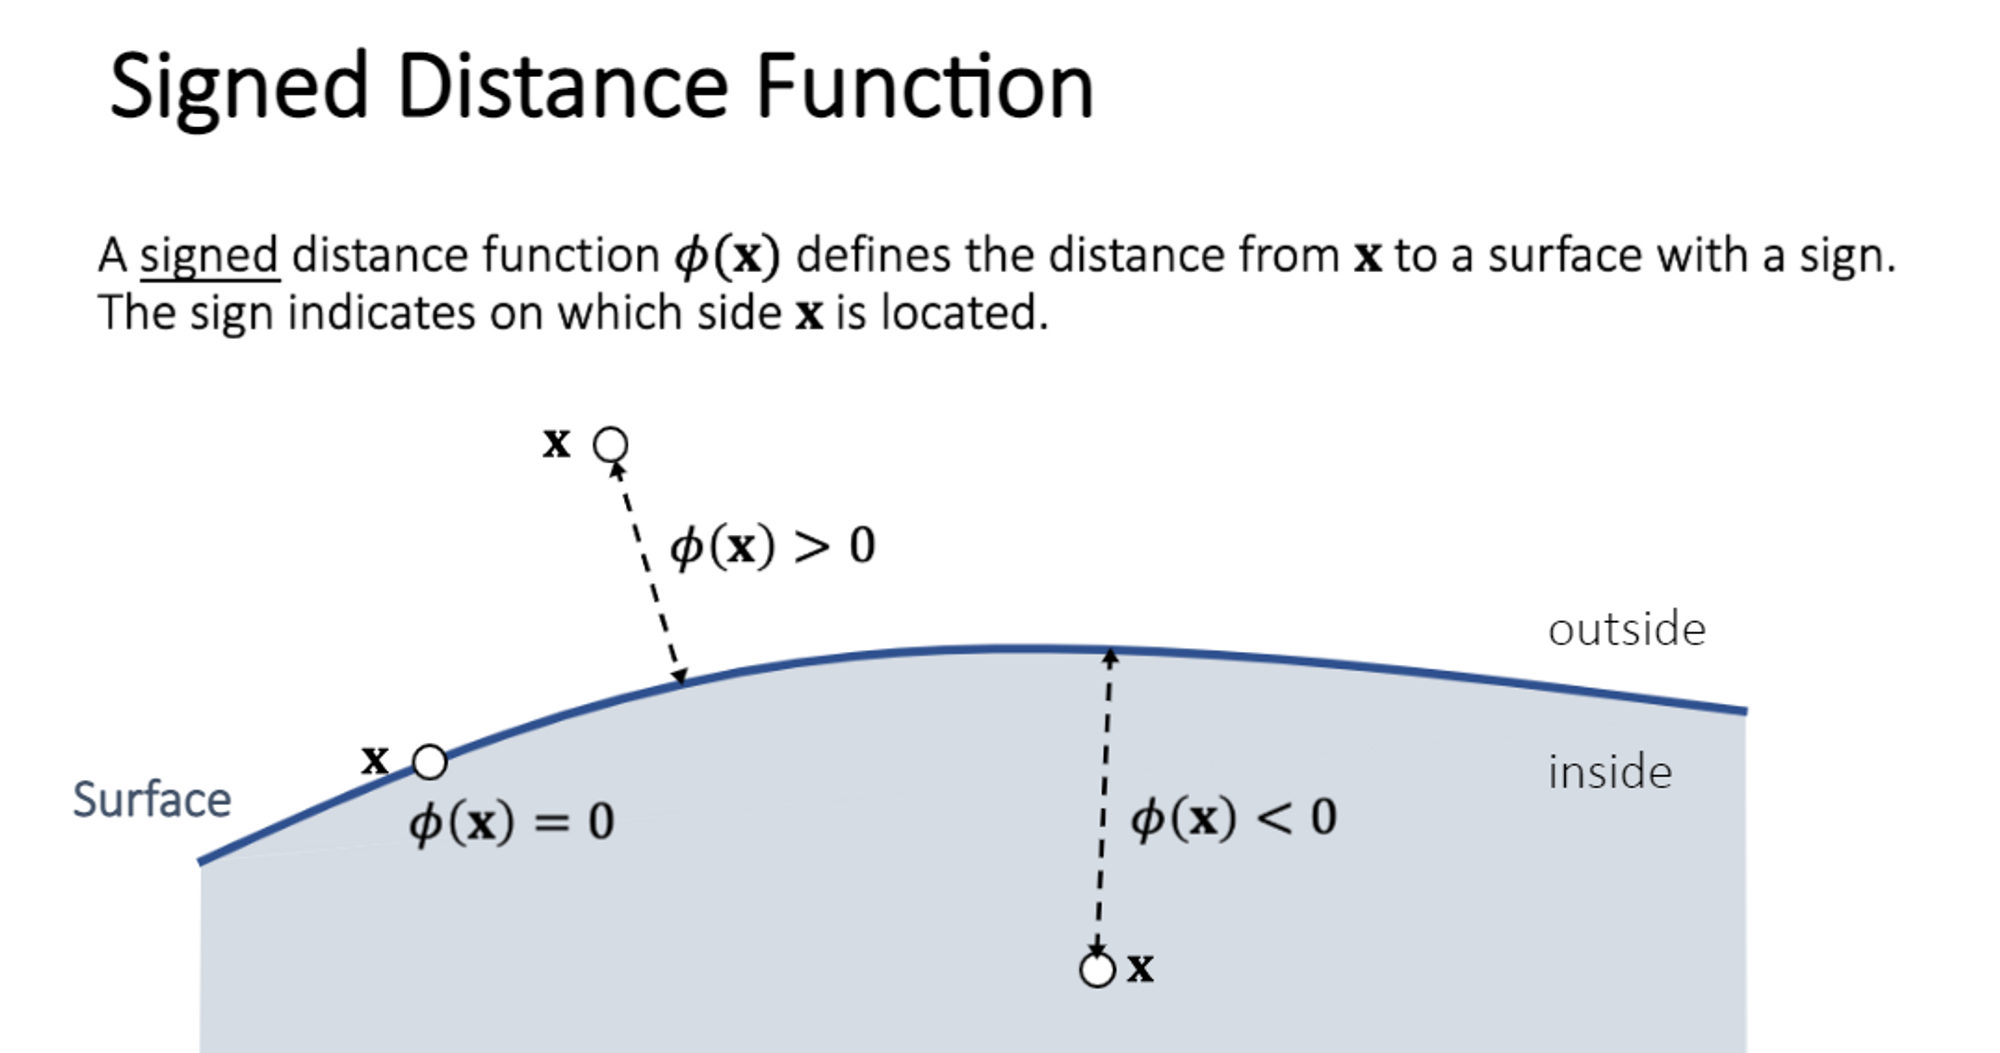
\includegraphics[width=\linewidth]{Signed Distance Function.png}
	\caption{Signed Distance Function}
\end{figure}
\section{Collision Handling}
Before considering rigid body collisions, we consider the simpler problem of how to judge the collision of a particle with other objects, and how this collision should be handled once it has been detected.
\subsection{Impulse Method}
As long as detecting an incoming object ($\phi(x)<0)$, we need to move it to the object surface, updating $x^{new}=x+|\phi(x)|N$, where $N$ is the nearest direction from the point to the surface.\\
And then we go ahead and check whether the velocity is pointing inside the object, if $v\cdot N \geq0$, it means that the velocity of the particle has been modified in the previous time step, and it's already going out, and we don't need to do anything about it.\\
Otherwise, when $v\cdot N \leq 0$, we need to decompose it orthogonally and recalculate its tangent and normal vectors as $v_N=-\mu_Nv_N/v_T=av_T$, where $a,\mu_N \in[0,1]$.
\begin{figure}[htb]
	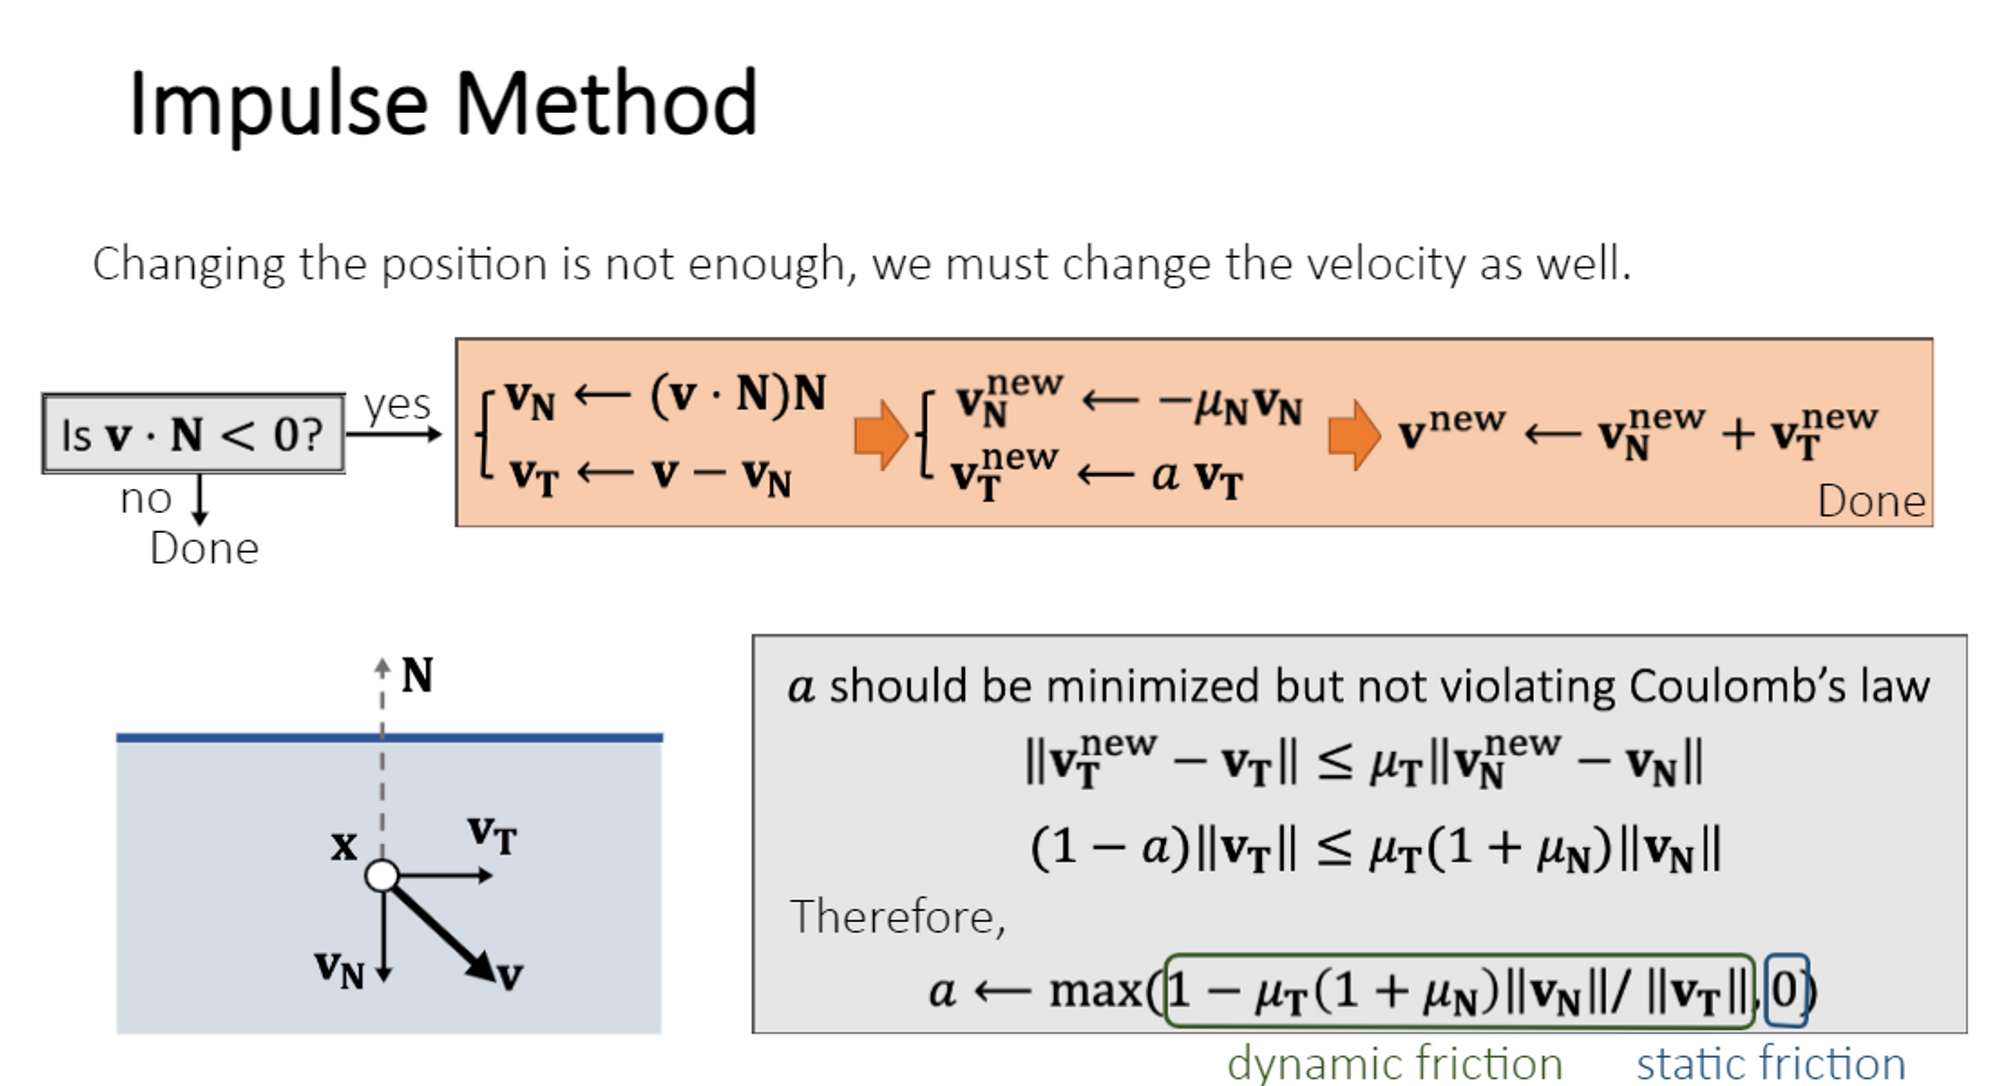
\includegraphics[width=\linewidth]{Impulse Method.png}
	\caption{Impulse Method}
\end{figure}
\subsection{State Update}
For each point that enters the object, we can get an impulse by calculating its new velocity and its previous velocity: $v_i^{new}-v_i=KJ$. By averaging these impulses, we are able to obtain a new impulse for the whole object, which in turn calculates the movement and position change of the object.
\begin{cpp}

x += fixed_delta_time * v;
Quat wq = Quat(w.x, w.y, w.z, 0);
Quat temp_q = wq * q;
q.x += 0.5f * fixed_delta_time * temp_q.x;
q.y += 0.5f * fixed_delta_time * temp_q.y;
q.z += 0.5f * fixed_delta_time * temp_q.z;
q.w += 0.5f * fixed_delta_time * temp_q.w;
object->transform->SetPos(x);
object->transform->SetRotation(glm::normalize(q));
\end{cpp}
\section{Results}
Finally, we build two scenes to detect the collision effect of a massive number of spherical rigid bodies. In rare cases, penetration of individual spheres may occur, but in most cases, it can reach a realistic physical simulation.\\\\
\begin{figure}[htb]
	\subfigure{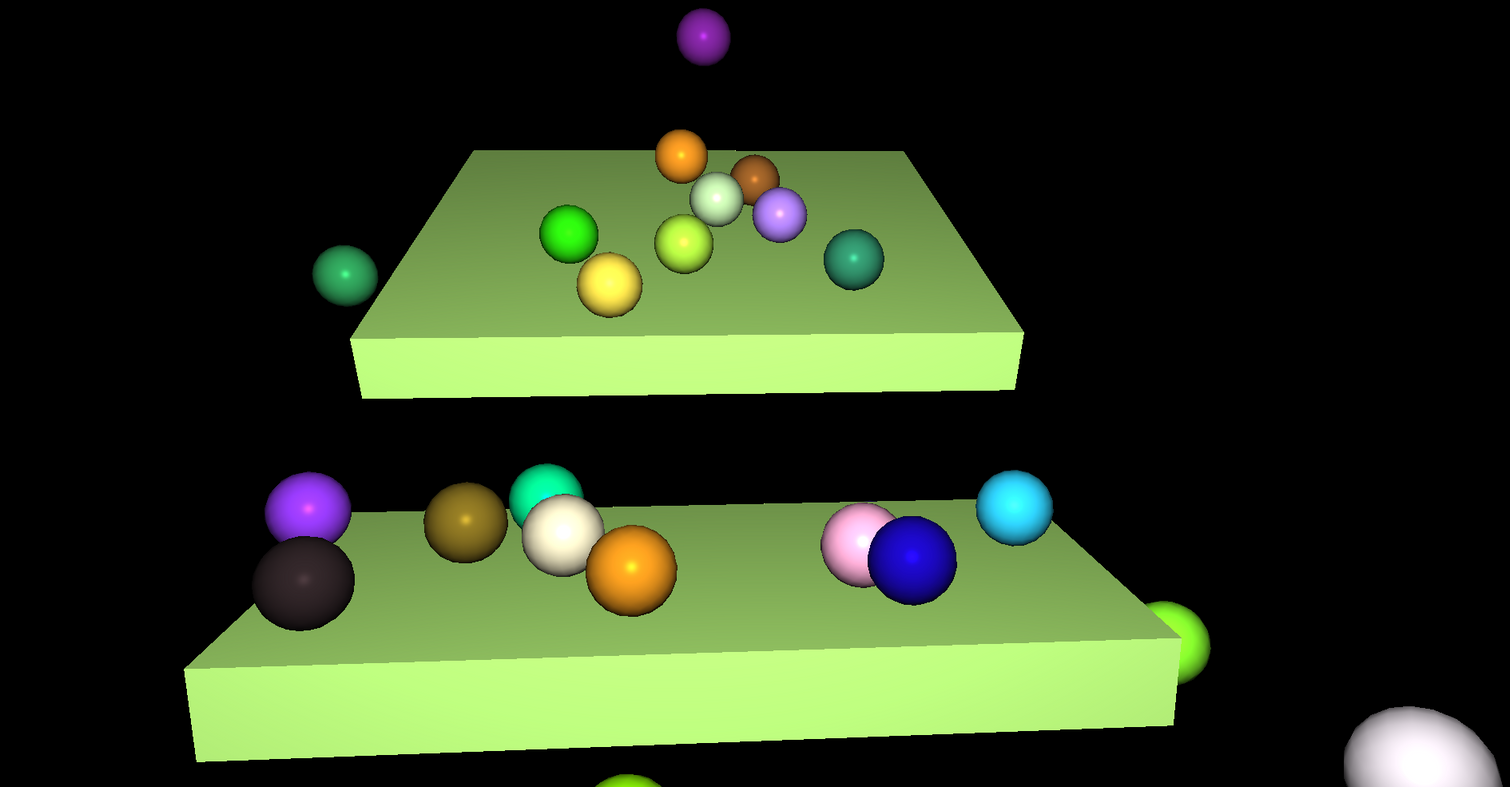
\includegraphics[width=0.49\linewidth]{ball1.png}}
	\subfigure{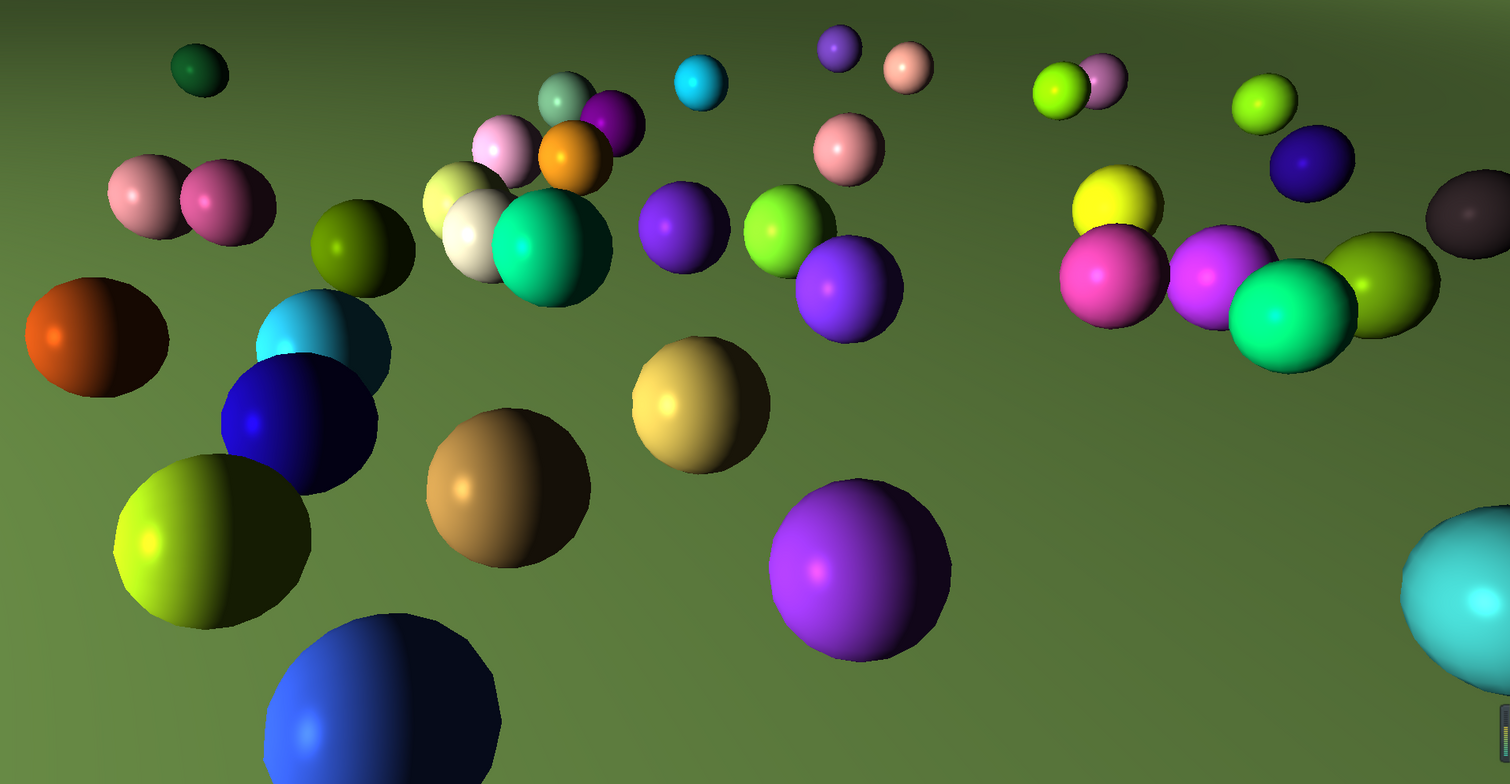
\includegraphics[width=0.49\linewidth]{ball2.png}}
	\caption{Ball}
\end{figure}
In addition, we are not limited to only spherical rigid bodies. We have tested a rabbit model by giving it initial velocity and angular velocity to detect the collision with the wall, which also has a good effect.
\begin{figure}[htb]
	\subfigure{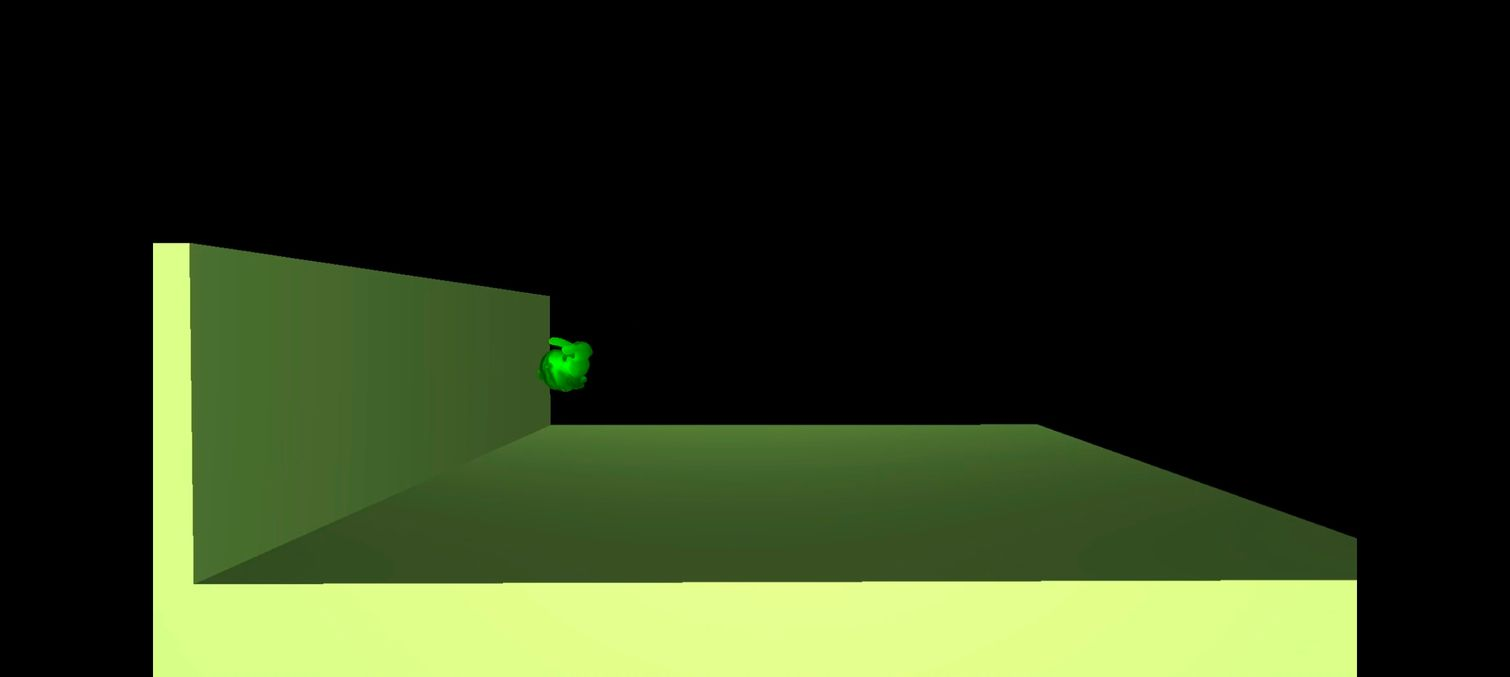
\includegraphics[width=0.49\linewidth]{bunny1.jpeg}}
	\subfigure{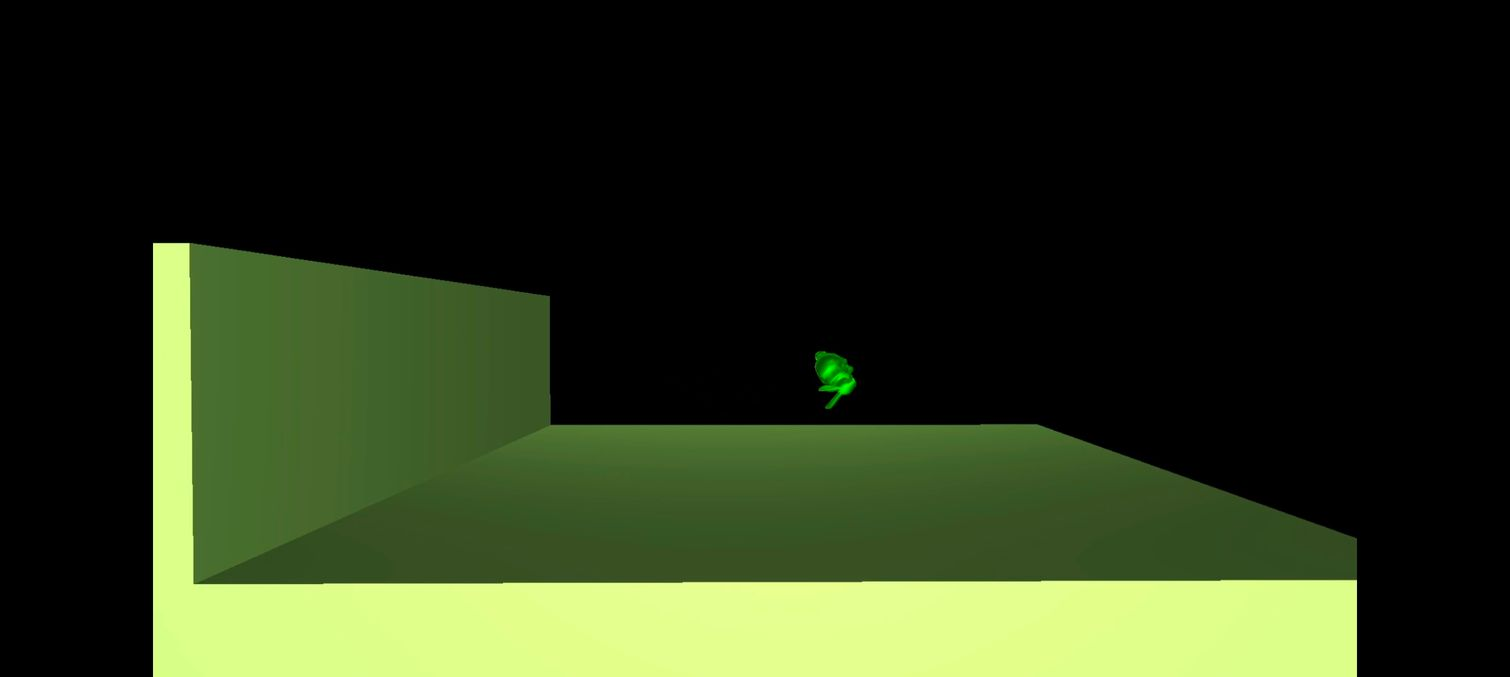
\includegraphics[width=0.49\linewidth]{bunny2.jpeg}}
	\caption{Bunny}
\end{figure}
\section{Contribution}
In this project, both of our teammates earnestly studied the physics and mathematics knowledge related to rigid bodies, and actively participated in the discussion of code architecture and code writing. Our main responsibilities for each other are listed below:
\begin{itemize}
	\item Ye HengWei: Impulse Method(In Unity & C++), Ball & Wall Collision, AABB, Bug Fix
	\item Shao KuiXiang: Scene Generation, Model Import, Ball & Ball Collision, Code Refactoring
\end{itemize}
% pictures should be in
\end{document}
